% C.37 直角△, ∠C=90, ∠A=30, BC=4
\documentclass[tikz,border=4pt]{standalone}
\usepackage{ctex}
\usepackage{amsmath}
\usetikzlibrary{calc, arrows.meta}
\begin{document}
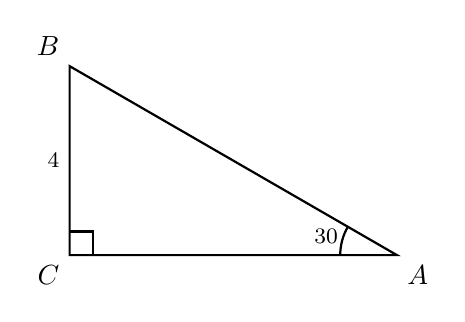
\begin{tikzpicture}[scale=0.6, thick]
  % BC=4 (opposite A=30). AC = BC/tan30 = 4/(1/√3)=4√3. AB = 2*BC = 8.
  \coordinate (C) at (0,0);
  \coordinate (A) at ({4*sqrt(3)},0);
  \coordinate (B) at (0,4);
  \draw (A) -- (C) -- (B) -- cycle;
  \draw (0.5,0)--(0.5,0.5)--(0,0.5);
  \node[below left] at (C) {$C$};
  \node[below right] at (A) {$A$};
  \node[above left] at (B) {$B$};
  \node[font=\footnotesize, left] at (0,2) {$4$};
  \draw ({4*sqrt(3)-1.2},0) arc (180:150:1.2);
  \node[font=\footnotesize] at ({4*sqrt(3)-1.5},0.4) {$30°$};
\end{tikzpicture}
\end{document}
